\documentclass[crop,tikz]{standalone} 
\usepackage{tikz, amsmath, amssymb, graphicx} 

\DeclareMathAlphabet\mathbfcal{OMS}{cmsy}{b}{n}

\newcommand{\Mt}{\mathbfcal{M}}
\newcommand{\Yt}{\mathbfcal{Y}}
\newcommand{\Ft}{\mathbfcal{F}}

\usetikzlibrary{positioning, shapes.geometric} 

\begin{document}  

\tikzset{fontscale/.style = {font=\relsize{#1}}
    }

\begin{tikzpicture} 

 
\node[inner sep=0pt] at (0, 0) {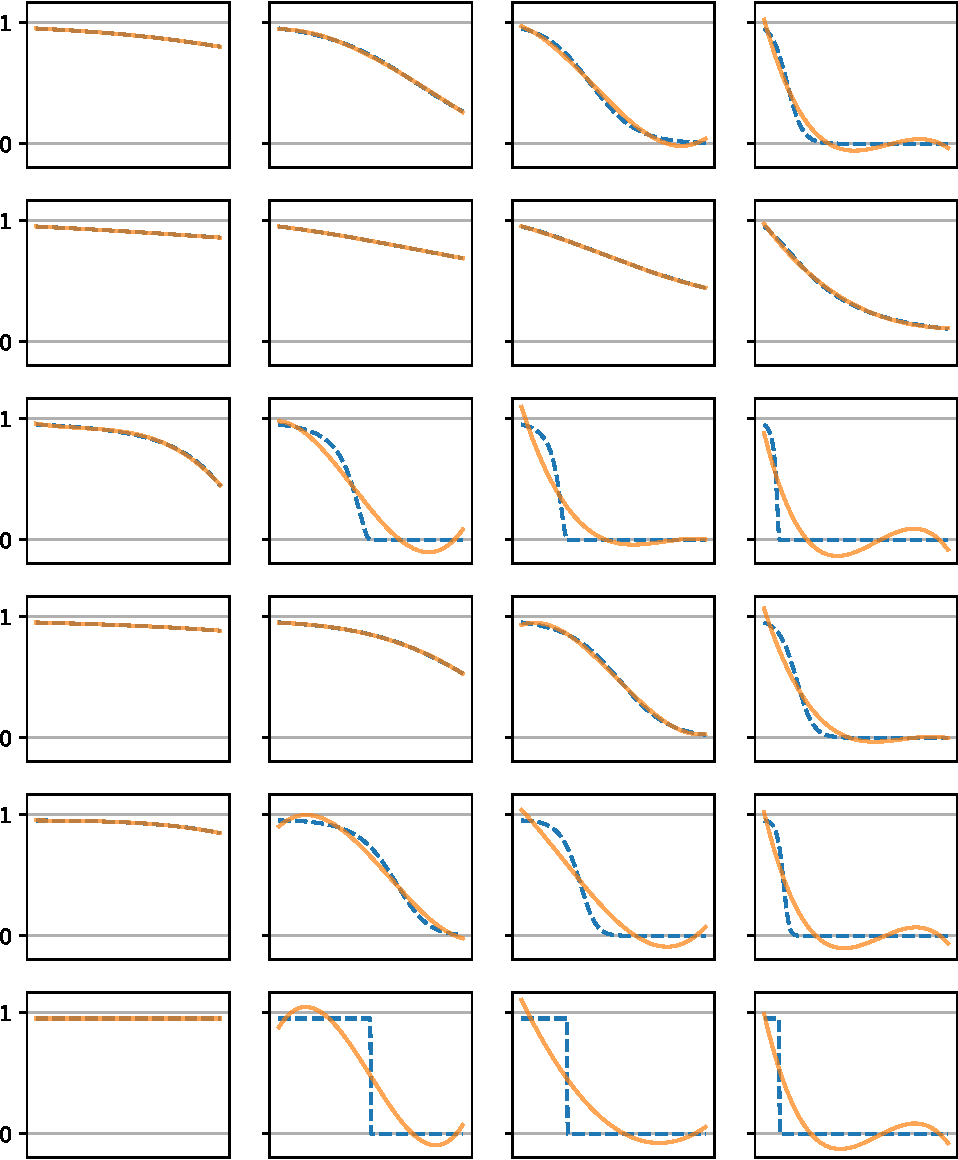
\includegraphics[width=.4\textwidth]{cheb_approx_raw.pdf}};

\node[inner sep=0pt, scale=0.4] at (-1.8, 3.1) {$\beta=0.2$};
\node[inner sep=0pt, scale=0.4] at (-0.58, 3.1) {$\beta=0.5$};
\node[inner sep=0pt, scale=0.4] at (0.66, 3.1) {$\beta=1$};
\node[inner sep=0pt, scale=0.4] at (1.89, 3.1) {$\beta=3$};

\node[inner sep=0pt, scale=0.4] at (-2.95, 2.53) {Diffusion};
\node[inner sep=0pt, scale=0.4] at (-2.95, 1.52) {1-Hop};
\node[inner sep=0pt, scale=0.4] at (-2.95, 0.5) {ReLu};
\node[inner sep=0pt, scale=0.4] at (-2.95, -0.5) {Sigmoid};
\node[inner sep=0pt, scale=0.4] at (-2.95, -1.5) {Gaussian};
\node[inner sep=0pt, scale=0.4] at (-2.95, -2.5) {Bandlimited};

\end{tikzpicture}
\end{document} 